\documentclass[journal=jacsat,manuscript=article,layout=onecolumn]{achemso}
\usepackage[version=3]{mhchem} % Formula subscripts using \ce{}
\usepackage[T1]{fontenc}       % Use modern font encodings
\usepackage{amsmath}
% NB added command for in line cite
\newcommand{\onlinecite}[1]{\hspace{-1 ex} \nocite{#1}\citenum{#1}} 
% 2 column equations
\usepackage{widetext, widetable}
%
\author{Z.~Levey}
\author{B.~A.~Laws}
\email{B.Laws@unsw.edu.au}
\author{K.~Nauta} 
\author{T.~Schmidt}

\affiliation{School of Chemistry, University of New South Wales, Sydney NSW 2052, Australia}
\title{Formation of PhenRad via CH ring insertion...}
\abbreviations{PES,PAD,EA,eKE,FWHM,VMI}
\DeclareUnicodeCharacter{2192}{-}
\begin{document} 
\begin{abstract} 
This is the manuscripts abstract...
\end{abstract} 
%\begin{tocentry}
%\includegraphics[width=1\textwidth]{Figures/TOC}
%\end{tocentry}

\section{Introduction}

The formation mechanism of polycyclic aromatic hydrocarbons (PAHs) is an increasingly important area of research due to their role in combustion, atmospheric, circumstellar, and interstellar chemistry. Incomplete combustion of hydrocarbon fuels results in the formation of soot particles which, when released into the atmosphere, contribute to global warming and environmental damage~\cite{bon13,ram08,shr10,fin97}. Inhalation and ingestion of these particles is also of concern for human health due to their toxic and carcinogenic properties~\cite{tiw15,tiw17,lah13,ame14}. PAHs are suspected to play the role of early intermediates in the soot nucleation process~\cite{fre02,wan11}. Comparably with terrestrial soot, PAHs are viewed as the initial precursors of stellar dust grains being formed in the circumstellar shells of carbon rich evolved stars~\cite{hen98,jag09,dra01,dra07}. The most convincing evidence for the presence of PAHs in the interstellar medium (ISM) comes from infrared emission features termed the aromatic infrared bands (AIBs). These strong features between 3-20um are ubiquitous in the spectra of interstellar objects and are characteristic of large PAH molecules~\cite{tie13,pec02}. Modelling based on these optical observations allows the inference of chemical abundances and size distributions with an estimated 20\% of the total cosmic carbon abundance locked up in PAHs of sizes 50—100 C atoms~\cite{tie08,dwe97}. PAHs are also strongly considered as carriers of the diffuse interstellar bands (DIBs) – a series of unidentified absorption features in the visible to near-infrared region~\cite{cox11}. Aromatic species such as benzene and benzonitrile, as well as fullerenes, C$_{60}$ (in its neutral and cationic state) and C$_{70}$, have been identified in the ISM through spectroscopic techniques~\cite{cer01,mcg18,cam10,cam15}, however, there has not yet been an identification of PAHs in the ISM. 

Due to the diversity of physical conditions within the ISM, the formation mechanism for interstellar PAHs is ambiguous. Current astrochemical models of PAH formation are predominately derived from combustion chemistry models. Bottom-up molecular growth processes in hot and dense circumstellar envelopes of carbon-rich asymptotic giant branch stars are largely based on the hydrogen abstraction-acetylene addition (HACA) mechanism~\cite{tie13}. HACA was first described as an activation of a radical site by H-abstraction/addition followed by sequential addition of acetylene, finally resulting in ring closure~\cite{fre85} and has been shown to occur experimentally for the formation of naphthalene from benzene via the phenylacetylene intermediate~\cite{par14,yan16}. However, there are some inherent shortcomings of this mechanism. Notably, modelling studies have reported that HACA under-predicts the concentration of PAHs in flames~\cite{raj12}. Also, the injection of PAHs from stellar sources occurs on a time scale that is significantly longer than the destruction of PAHs caused by interstellar shockwaves and bombardment by energetic cosmic rays suggesting that crucial PAH growth routes are missing within the astrochemical model~\cite{mic10a,mic10b,mic11}. Alternate PAH formation mechanisms have been proposed in conjunction with HACA to account for the deficiencies in PAH concentrations. These include the recombination of resonance stabilized radicals (RSRs)~\cite{mel96,mil92,joh18}, condensation of small PAHs~\cite{sie00}, phenyl addition/cyclization (PAC)~\cite{shu08} and methyl addition/cyclization (MAC)~\cite{shu10}.

Acenaphthylene (ACYN) is considered the first significant island of stability “pulling” the HACA sequence forward~\cite{fre20}. Theoretical investigations of the reaction between 1-naphthyl radical and acetylene at elevated temperatures above 1000 K show predominant formation of ACYN over phenanthrene and anthracene. Rapid cyclization after the addition of a single acetylene molecule adjacent to the bay region of a PAH to form a five-membered ring occurs much faster than the addition of a second acetylene, followed by cyclization to form a third aromatic ring~\cite{kis13}.  It was shown that PAHs with exclusively six-membered rings accounted for $\leq$ 6\% of the total yield from the reaction of naphthalene and acetylene, with most products containing a five-membered ring ($\sim$75\%). Hence, a mechanism converting a five-member ring on the edge of a PAH molecule to a six-member ring is necessary to explain reaction pathways to tricyclic and larger PAHs.

Ring expansion has been thoroughly investigated for an isolated five-member ring, the cyclopentadienyl radical~\cite{mel96,mos96,sha09}, and a five-member ring attached to benzene, the 1-indenyl radical~\cite{meb16,jas13,zha19}. This reaction can readily occur by methylation (addition of a CH$_3$ radical) to form benzene and naphthalene, respectively. Additionally, expansion of a five-member ring to a six-member ring has been demonstrated through the reaction of pyrrole with methylidyne radical (CH) to form pyridine~\cite{soo10}. The CH radical in its ground state has been detected in combustion environments~\cite{lov11,tin11,zha12}, the interstellar medium~\cite{ger10} and under plasma conditions~\cite{zho06}. Reactions between the CH radical and small unsaturated hydrocarbons and carbonyls can result in CH insertion to the C—C $\pi$-bond through a cyclic intermediate (cycloaddition) followed by ring-opening isomerization~\cite{gou09,tre13,gou12,tre16}. Isotopomer distribution experiments provided additional evidence for this cycloaddition mechanism through the reactions of deuterated methylidyne radical (CD) with ethylene and pyrrole~\cite{gou09,soo10}. Recently, ab initio calculations in combination with RRKM-ME calculations for the reaction of 1-acenaphthyl and methyl radicals exhibit ring expansion of the five-member ring by methylation to produce the phenalenyl radical~\cite{por20}. The phenalenyl radical is an open-shell, neutral, RSR consisting of three benzene rings fused together by a central carbon atom. It is considered a prototypical open-shell graphene fragment~\cite{mor11} and is posited to have a role in soot inception and growth~\cite{joh18}. The gas phase, resonance enhanced multi-photon ionisation (REMPI) spectrum for the D$_0$ $\rightarrow$ D$_1$ state of the phenalenyl radical has been previously recorded~\cite{oco11}. 

In this work, we experimentally investigated the ring-expansion PAH growth mechanism for ACYN to phenalenyl radical. ACYN and methane (CH$_4$) molecules interact and undergo subsequent radical gas-phase reactions induced by means of an electrical discharge. This allowed for the simultaneous examination of the methylation and cycloaddition mechanisms previously described. The reaction products and intermediates were identified using the mass selective REMPI techinque in conjunction with isotope labelling experiments. We determined that ACYN formed the phenalenyl radical through a cycloaddition CH insertion reaction.  





\section{Results}
Here is a figure. You can then refer to the figure using Fig.~\ref{fig1-delay}.
\begin{figure}
	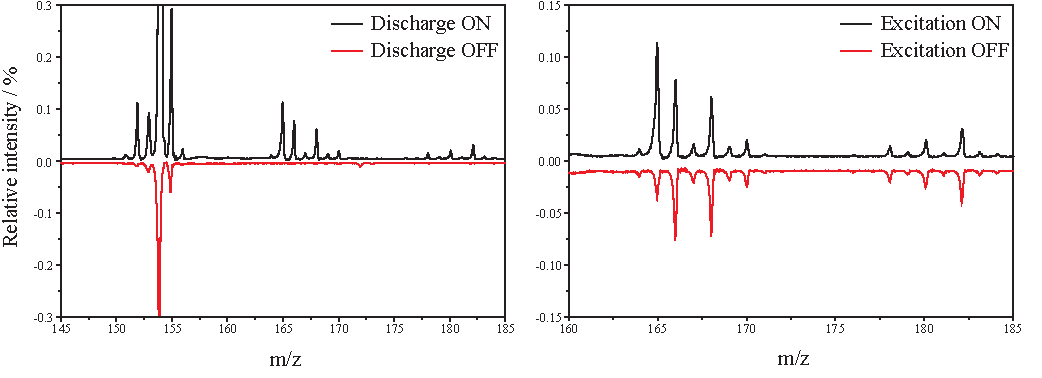
\includegraphics[width=1\textwidth]{Figures/discharge-exc}
	\caption{A figure showing the depletion rate for different laser delays.}
	\label{fig1-delay}
\end{figure}

\begin{figure}
	\includegraphics[width=0.5\textwidth]{Figures/CHinsertion/ArVsCD4}
	\caption{A figure showing the depletion rate for different laser delays.}
	\label{fig1-delay}
\end{figure}

\section{Discussion}
Equations may be written using general LaTeX format, and the same labelling method.
\begin{equation}
I(\theta,\epsilon) = \frac{\sigma_{\text{total}}(\epsilon)}{4\pi}[1+\beta(\epsilon)\text{P}_2(\cos\theta)],
\label{eq:beta}
\end{equation}
where $\beta$ in Eq.~(\ref{eq:beta}) is a really cool parameter.

We can also make tables, like this one, Table~\ref{tab:C2H}.
\begin{table}
	\caption{This is my table caption.} \label{tab:C2H}
	\begin{tabular}{c c c c c}
		\hline Peak & eBE (cm$^{-1}$) & $v$ (cm$^{-1}$) & $\beta$ & Symmetry \\ 
		& & & & \\\hline \hline
		& 23 591 & -231 & + & $\Sigma^+$ 
	\end{tabular}
\end{table}

\section{Conclusion}

\section{Experimental Details}


\begin{acknowledgement}
	This research was supported by the Australian Research Council Discovery
	Project Grant DP160102585. The author's thank Andrei Sanov for discussion on his modified Cooper-Zare anisotropy model.
\end{acknowledgement}


% Create the reference section using BibTeX: 
\bibliography{PhenRad}

%\newpage
%\onecolumn
%\subsection{TOC Graphic}
%\vspace{2ex}
%\begin{center}
%	\includegraphics[width=8.5cm]{Figures/TOC}
%\end{center}


\end{document}
